% =====================================================================
%  Livelli di Fermi in un IGBT: stato di riposo, blocco e conduzione
% =====================================================================
\documentclass[11pt,a4paper]{article}

\usepackage[T1]{fontenc}
\usepackage[utf8]{inputenc}
\usepackage[margin=2.4cm]{geometry}
\usepackage{amsmath,amssymb}
\usepackage{booktabs}
\usepackage{enumitem}
\usepackage{float}
\usepackage{xcolor}
\usepackage{tikz}
\usepackage{caption}
\usepackage{subcaption}
\usepackage[hidelinks]{hyperref}
\usetikzlibrary{arrows.meta,patterns,positioning,calc,decorations.pathreplacing}

% ---------------------------------------------------------------- stili
\definecolor{ncol}{RGB}{20,70,160}
\definecolor{pcol}{RGB}{170,30,30}
\definecolor{oxcol}{RGB}{200,160,20}

\tikzset{
  Eband/.style   = {line width=1.0pt, black},
  Emid/.style    = {line width=0.4pt, black!45, dash pattern=on 1.5pt off 1.5pt},
  Ef/.style      = {line width=0.9pt, black!70, dashed},
  Efn/.style     = {line width=0.9pt, ncol, dashed},
  Efp/.style     = {line width=0.9pt, pcol, dashed},
  sep/.style     = {line width=0.3pt, black!30, dotted},
  reglab/.style  = {font=\scriptsize\sffamily, black!70},
  enlab/.style   = {font=\scriptsize},
  eflow/.style   = {-{Latex[length=2mm]}, ncol, line width=0.8pt},
  hflow/.style   = {-{Latex[length=2mm]}, pcol, line width=0.8pt},
}

% comodo: energy gap del silicio usato nei disegni (eV)
\newcommand{\EG}{1.12}

\title{\bfseries Livelli di Fermi in un IGBT\\[2pt]
\large Stato di riposo, stato di blocco e stato di conduzione}
\author{}
\date{}

\begin{document}
\maketitle
\vspace{-2.2\baselineskip}

\section{Struttura e principio di funzionamento}

L'IGBT (\emph{Insulated Gate Bipolar Transistor}) a canale n e' un dispositivo
verticale a quattro strati $\mathrm{p^{+}\,n\,n^{-}\,p}$ con un MOSFET a gate
isolato integrato sulla superficie. Dal punto di vista circuitale equivale a un
MOSFET a canale n che pilota la base di un transistore bipolare PNP:

\begin{itemize}[nosep,leftmargin=1.4em]
  \item il \textbf{MOSFET} (sorgente $\mathrm{n^{+}}$, p-body, gate su ossido)
        fornisce il controllo in tensione e inietta \emph{elettroni} nella
        regione di drift;
  \item il \textbf{PNP} (emettitore $\mathrm{p^{+}}$ di collettore, base
        $\mathrm{n^{-}}$ di drift, collettore p-body) inietta \emph{lacune}
        nella drift dal lato collettore.
\end{itemize}

La contemporanea presenza di elettroni e lacune nella regione $\mathrm{n^{-}}$
produce la \emph{modulazione della conduttivita'}: la densita' di plasma
($n \simeq p \sim 10^{16}\!-\!10^{17}\,\mathrm{cm^{-3}}$) supera di due o tre
ordini di grandezza il drogaggio della drift
($N_D \sim 10^{13}\!-\!10^{14}\,\mathrm{cm^{-3}}$), riducendo drasticamente la
caduta resistiva rispetto a un MOSFET di pari tensione di blocco. Il prezzo da
pagare e' la tensione di soglia di giunzione ($\approx 0{,}7$--$0{,}9$~V) sempre
presente in serie e la coda di corrente allo spegnimento, dovuta alla
ricombinazione del plasma immagazzinato.

\begin{figure}[H]
\centering
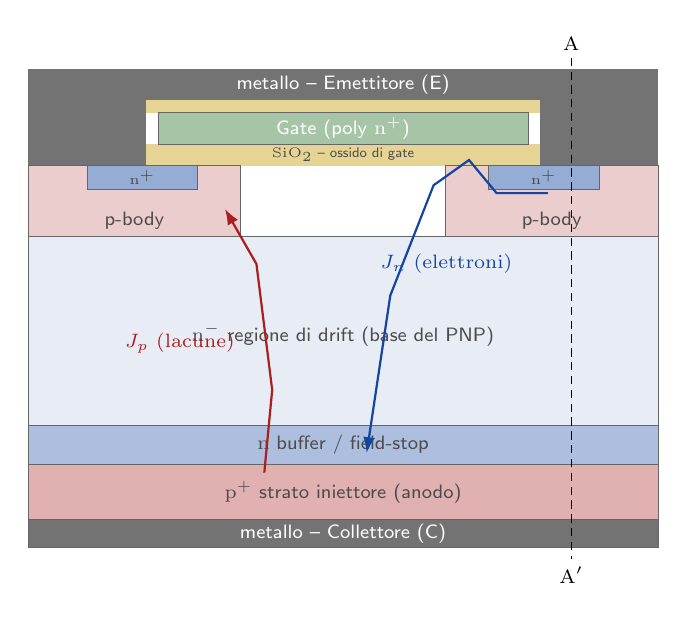
\begin{tikzpicture}[x=1cm,y=1cm]
% --- regioni
\fill[black!55]      (0,0)      rectangle (8,0.35);   % metallo collettore
\fill[pcol!35]       (0,0.35)   rectangle (8,1.05);   % p+ collector (anodo)
\fill[ncol!35]       (0,1.05)   rectangle (8,1.55);   % n buffer
\fill[ncol!10]       (0,1.55)   rectangle (8,3.95);   % n- drift
\fill[pcol!22]       (0,3.95)   rectangle (2.7,4.85); % p-body sx
\fill[pcol!22]       (5.3,3.95) rectangle (8,4.85);   % p-body dx
\fill[ncol!45]       (0.75,4.55) rectangle (2.15,4.85); % n+ emitter sx
\fill[ncol!45]       (5.85,4.55) rectangle (7.25,4.85); % n+ emitter dx
\fill[oxcol!45]      (1.5,4.85) rectangle (6.5,5.12);  % gate oxide
\fill[green!35!black!35] (1.65,5.12) rectangle (6.35,5.52); % poly gate
\fill[oxcol!45]      (1.5,5.52) rectangle (6.5,5.68);  % dielettrico intermedio
\fill[black!55]      (0,5.68)   rectangle (8,6.08);    % metallo emettitore
\fill[black!55]      (0,4.85)   rectangle (1.5,5.68);  % contatto sx
\fill[black!55]      (6.5,4.85) rectangle (8,5.68);    % contatto dx

% --- contorni
\draw[black!60,line width=0.3pt]
  (0,0) rectangle (8,0.35) (0,0.35) rectangle (8,1.05)
  (0,1.05) rectangle (8,1.55) (0,1.55) rectangle (8,3.95)
  (0,3.95) rectangle (2.7,4.85) (5.3,3.95) rectangle (8,4.85)
  (0.75,4.55) rectangle (2.15,4.85) (5.85,4.55) rectangle (7.25,4.85)
  (1.65,5.12) rectangle (6.35,5.52);

% --- etichette regioni
\node[reglab,white] at (4,0.17) {metallo -- Collettore (C)};
\node[reglab] at (4,0.70) {$\mathrm{p^{+}}$ strato iniettore (anodo)};
\node[reglab] at (4,1.30) {$\mathrm{n}$ buffer / field-stop};
\node[reglab] at (4,2.70) {$\mathrm{n^{-}}$ regione di drift (base del PNP)};
\node[reglab] at (1.35,4.15) {p-body};
\node[reglab] at (6.65,4.15) {p-body};
\node[reglab,font=\tiny\sffamily] at (1.45,4.70) {$\mathrm{n^{+}}$};
\node[reglab,font=\tiny\sffamily] at (6.55,4.70) {$\mathrm{n^{+}}$};
\node[reglab,white] at (4,5.32) {Gate (poly $\mathrm{n^{+}}$)};
\node[reglab,white] at (4,5.88) {metallo -- Emettitore (E)};
\node[reglab,font=\tiny\sffamily] at (4,4.985) {$\mathrm{SiO_2}$ -- ossido di gate};

% --- percorsi dei portatori
\draw[eflow] (6.6,4.50) -- (5.95,4.50) -- (5.6,4.92) -- (5.15,4.60)
             -- (4.6,3.2) -- (4.3,1.2);
\node[enlab,ncol,anchor=west] at (4.35,3.6) {$J_n$ (elettroni)};
\draw[hflow] (3.0,0.95) -- (3.1,2.0) -- (2.9,3.6) -- (2.5,4.3);
\node[enlab,pcol,anchor=east] at (2.75,2.6) {$J_p$ (lacune)};

% --- linea di taglio A-A'
\draw[black,line width=0.6pt,dash pattern=on 3pt off 2pt]
      (6.9,6.22) -- (6.9,-0.15);
\node[enlab] at (6.9,6.40) {A};
\node[enlab] at (6.9,-0.35) {A$'$};
\end{tikzpicture}
\caption{Sezione schematica di una cella IGBT a canale n (planare). La linea
A--A$'$ individua il taglio verticale usato per i diagrammi a bande delle
Fig.~\ref{fig:eq}, \ref{fig:block} e \ref{fig:on}. Le proporzioni non sono in
scala: la drift $\mathrm{n^{-}}$ e' in realta' molto piu' spessa degli altri
strati.}
\label{fig:struttura}
\end{figure}

\section{Richiami: livello di Fermi e quasi-livelli di Fermi}

All'equilibrio termodinamico (nessuna tensione applicata, nessun gradiente di
temperatura, nessuna illuminazione) esiste \emph{un solo} livello di Fermi
$E_F$, ed esso e' \textbf{costante in tutto il dispositivo}. Le concentrazioni
di portatori sono

\begin{equation}
n = n_i \exp\!\left(\frac{E_F-E_i}{kT}\right),
\qquad
p = n_i \exp\!\left(\frac{E_i-E_F}{kT}\right),
\qquad
np = n_i^2 ,
\end{equation}

dove $E_i$ e' il livello intrinseco (circa a meta' gap). La posizione di $E_F$
rispetto a $E_i$ codifica il drogaggio locale: vicino a $E_C$ nelle zone n,
vicino a $E_V$ nelle zone p. Poiche' $E_F$ deve restare orizzontale, sono le
\emph{bande} a piegarsi in corrispondenza delle giunzioni: la piegatura vale
$qV_{bi}$, con
\begin{equation}
V_{bi} = \frac{kT}{q}\,\ln\!\frac{N_A N_D}{n_i^{2}} \approx 0{,}7\!-\!0{,}9~\mathrm{V}
\quad\text{per le giunzioni tipiche di un IGBT.}
\end{equation}

Fuori equilibrio (polarizzazione applicata, corrente che scorre) elettroni e
lacune non sono piu' in equilibrio fra loro. Si introducono allora i
\textbf{quasi-livelli di Fermi} $E_{Fn}$ ed $E_{Fp}$:

\begin{equation}
n = n_i \exp\!\left(\frac{E_{Fn}-E_i}{kT}\right),\qquad
p = n_i \exp\!\left(\frac{E_i-E_{Fp}}{kT}\right),\qquad
\boxed{\;np = n_i^{2}\exp\!\left(\frac{E_{Fn}-E_{Fp}}{kT}\right)\;}
\end{equation}

La loro separazione ha un significato fisico immediato:
\begin{itemize}[nosep,leftmargin=1.4em]
  \item $E_{Fn}-E_{Fp} = 0$: equilibrio locale ($np=n_i^2$);
  \item $E_{Fn}-E_{Fp} > 0$: iniezione (giunzione polarizzata direttamente),
        $np > n_i^2$;
  \item $E_{Fn}-E_{Fp} < 0$: estrazione (giunzione polarizzata inversamente),
        $np < n_i^2$;
  \item la differenza $E_{Fn}-E_{Fp}$ misurata ai due contatti vale
        esattamente $qV_{applicata}$.
\end{itemize}

Infine, i quasi-livelli sono i veri potenziali che guidano il trasporto: le
densita' di corrente si scrivono in forma compatta (deriva + diffusione
inglobate) come

\begin{equation}
J_n = \mu_n\, n\, \frac{\mathrm{d}E_{Fn}}{\mathrm{d}x},
\qquad
J_p = \mu_p\, p\, \frac{\mathrm{d}E_{Fp}}{\mathrm{d}x}.
\end{equation}

Un quasi-livello \emph{orizzontale} significa quindi corrente nulla per quel
tipo di portatore; la sua \emph{pendenza} e' proporzionale alla corrispondente
densita' di corrente divisa per la concentrazione locale.

\section{Stato di riposo (\texorpdfstring{$V_{GE}=0$, $V_{CE}=0$}{VGE=0, VCE=0})}

Con entrambi i terminali cortocircuitati il dispositivo e' in equilibrio
termodinamico. Vale un unico $E_F$ orizzontale, mentre le bande si piegano in
corrispondenza delle tre giunzioni interne (Fig.~\ref{fig:eq}):

\begin{itemize}[nosep,leftmargin=1.4em]
  \item $\mathrm{n^{+}}$ emettitore / p-body: barriera di circa $0{,}85$~eV, che
        impedisce agli elettroni della sorgente di entrare nel body;
  \item p-body / $\mathrm{n^{-}}$ drift (giunzione $J_2$, quella che sostiene la
        tensione in blocco): la zona svuotata e' fortemente asimmetrica e si
        estende quasi tutta nella drift poco drogata;
  \item $\mathrm{n}$ buffer / $\mathrm{p^{+}}$ collettore (giunzione $J_1$,
        quella che inietta le lacune in conduzione).
\end{itemize}

Non c'e' corrente perche' i due contatti si trovano allo stesso potenziale
elettrochimico: le componenti di deriva e di diffusione a ogni giunzione si
bilanciano esattamente. Il dispositivo e' bloccante in entrambi i sensi:
$J_2$ blocca la tensione diretta, $J_1$ quella inversa.

\begin{figure}[H]
\centering
% ---- coordinate delle bande all'equilibrio ------------------------
\def\EcEq{(0,0.06) (1.0,0.06) (1.2,0.22) (1.5,0.62) (1.8,0.86) (2.1,0.90)
           (3.0,0.90) (3.3,0.86) (3.7,0.66) (4.3,0.36) (4.8,0.27) (5.3,0.25)
           (8.2,0.25) (8.5,0.18) (8.9,0.12) (9.4,0.12) (9.7,0.36) (10.0,0.76)
           (10.3,0.96) (10.6,1.00) (11.0,1.00)}
\begin{tikzpicture}[x=0.85cm,y=1.55cm]
% separatori di regione
\foreach \x in {1.2,3.2,8.4,9.4} \draw[sep] (\x,-1.25) -- (\x,1.30);
% etichette regioni
\node[reglab] at (0.6,1.42)  {$\mathrm{n^{+}}$};
\node[reglab] at (2.2,1.42)  {p-body};
\node[reglab] at (5.8,1.42)  {$\mathrm{n^{-}}$ drift};
\node[reglab] at (8.9,1.42)  {buffer};
\node[reglab] at (10.2,1.42) {$\mathrm{p^{+}}$};
% bande
\draw[Eband] plot[smooth,tension=0.55] coordinates {\EcEq};
\draw[Eband,shift={(0,-\EG)}] plot[smooth,tension=0.55] coordinates {\EcEq};
\draw[Emid,shift={(0,-0.56)}] plot[smooth,tension=0.55] coordinates {\EcEq};
% livello di Fermi
\draw[Ef] (-0.2,0) -- (11.2,0);
% etichette energie
\node[enlab,anchor=west] at (11.15,1.00) {$E_C$};
\node[enlab,anchor=west] at (11.15,-0.12) {$E_V$};
\node[enlab,anchor=west] at (11.15,0.44) {$E_i$};
\node[enlab,anchor=east,black!70] at (-0.25,0) {$E_F$};
% quote barriere
\draw[<->,>=Latex,black!60,line width=0.4pt] (3.05,0.90) -- (3.05,0.25);
\node[enlab,anchor=west,black!60] at (2.55,0.60) {\;$qV_{bi,2}$};
\draw[<->,>=Latex,black!60,line width=0.4pt] (9.55,1.00) -- (9.55,0.12);
\node[enlab,anchor=west,black!60] at (9.6,0.60) {$qV_{bi,1}$};
\end{tikzpicture}
\caption{Stato di riposo ($V_{GE}=V_{CE}=0$): equilibrio termodinamico lungo il
taglio A--A$'$. Il livello di Fermi $E_F$ e' unico e perfettamente orizzontale;
tutta l'informazione sulle giunzioni e' contenuta nella piegatura delle bande.}
\label{fig:eq}
\end{figure}

\section{Stato di blocco (\texorpdfstring{$V_{GE}=0$, $V_{CE}>0$}{VGE=0, VCE>0})}

Applicando una tensione positiva sul collettore senza pilotare il gate, non
esiste canale: la giunzione $J_2$ (p-body/$\mathrm{n^{-}}$) si polarizza
inversamente e ne assorbe quasi tutta la tensione. Le bande della drift si
abbassano di $qV_{CE}$ rispetto al p-body e la zona svuotata si allarga
secondo
\begin{equation}
w_{dep} \simeq \sqrt{\frac{2\varepsilon_{Si}\,(V_{bi}+V_{CE})}{q N_D}} .
\end{equation}

Dal punto di vista dei livelli di Fermi accade il fatto caratteristico:
\textbf{$E_F$ si sdoppia}. $E_{Fp}$ resta agganciato al potenziale del contatto
di emettitore, $E_{Fn}$ a quello di collettore, e i due si separano di
$qV_{CE}$ (Fig.~\ref{fig:block}). All'interno della zona svuotata i due
quasi-livelli si incrociano; qui $E_{Fn}<E_{Fp}$, cioe' $np \ll n_i^2$: e' la
condizione di \emph{estrazione}, e la piccola corrente residua
$I_{CES}$ e' proprio la corrente di generazione termica nello spazio svuotato
(piu' la componente di guadagno del PNP, motivo per cui l'$I_{CES}$ di un IGBT
cresce rapidamente con la temperatura).

Il buffer $\mathrm{n}$ ha qui un ruolo preciso: arresta il fronte di campo
elettrico prima che raggiunga il $\mathrm{p^{+}}$ (\emph{punch-through} /
\emph{field-stop}), permettendo di usare una drift piu' sottile a parita' di
tensione nominale.

\begin{figure}[H]
\centering
\def\EcBl{(0,0.06) (1.0,0.06) (1.2,0.24) (1.5,0.64) (1.8,0.88) (2.1,0.90)
           (3.0,0.90) (3.3,0.72) (3.7,0.36) (4.1,0.02) (4.7,-0.48)
           (5.3,-0.92) (5.9,-1.28) (6.5,-1.54) (7.1,-1.70) (7.6,-1.75)
           (8.2,-1.76) (8.5,-1.84) (8.9,-1.88) (9.3,-1.88) (9.6,-1.62)
           (9.9,-1.20) (10.2,-1.02) (10.5,-1.00) (11.0,-1.00)}
\begin{tikzpicture}[x=0.85cm,y=1.05cm]
\foreach \x in {1.2,3.2,8.4,9.4} \draw[sep] (\x,-3.15) -- (\x,1.30);
\node[reglab] at (0.6,1.45)  {$\mathrm{n^{+}}$};
\node[reglab] at (2.2,1.45)  {p-body};
\node[reglab] at (5.8,1.45)  {$\mathrm{n^{-}}$ drift};
\node[reglab] at (8.9,1.45)  {buffer};
\node[reglab] at (10.2,1.45) {$\mathrm{p^{+}}$};
% zona svuotata
\fill[black!5] (3.2,-3.1) rectangle (7.8,1.2);
\node[reglab,anchor=west,align=left] at (5.9,-0.25) {zona svuotata\\($E$ massimo su $J_2$)};
% bande
\draw[Eband] plot[smooth,tension=0.55] coordinates {\EcBl};
\draw[Eband,shift={(0,-\EG)}] plot[smooth,tension=0.55] coordinates {\EcBl};
\draw[Emid,shift={(0,-0.56)}] plot[smooth,tension=0.55] coordinates {\EcBl};
% quasi-livelli
\draw[Efp] plot[smooth,tension=0.6] coordinates
  {(-0.2,0) (3.4,0) (4.0,-0.04) (4.5,-0.45) (5.0,-1.25) (5.5,-1.82)
   (6.0,-1.97) (6.6,-2.00) (11.2,-2.00)};
\draw[Efn] plot[smooth,tension=0.6] coordinates
  {(-0.2,0) (2.9,0) (3.3,-0.10) (3.7,-0.70) (4.2,-1.50) (4.7,-1.90)
   (5.2,-1.99) (5.8,-2.00) (11.2,-2.00)};
\node[enlab,anchor=east,ncol] at (-0.25,0.16) {$E_{Fn}$};
\node[enlab,anchor=east,pcol] at (-0.25,-0.18) {$E_{Fp}$};
\node[enlab,font=\tiny,anchor=south,fill=white,inner sep=1pt] at (7.0,-1.99)
      {\textcolor{ncol}{$E_{Fn}$}\,$=$\,\textcolor{pcol}{$E_{Fp}$}};
\node[enlab,anchor=west] at (11.15,-1.00) {$E_C$};
\node[enlab,anchor=west] at (11.15,-2.14) {$E_V$};
% quota qVce
\draw[<->,>=Latex,black!60,line width=0.4pt] (2.35,0) -- (2.35,-2.00);
\node[enlab,anchor=east,black!60] at (2.3,-1.0) {$qV_{CE}$};
\end{tikzpicture}
\caption{Stato di blocco ($V_{GE}=0$, $V_{CE}>0$). Il livello di Fermi si
sdoppia: $E_{Fn}$ ed $E_{Fp}$ differiscono di $qV_{CE}$ fra i due contatti.
Praticamente tutta la caduta e' sostenuta dalla giunzione $J_2$; nella zona
svuotata $E_{Fn}<E_{Fp}$ ($np\ll n_i^2$). Il valore di $V_{CE}$ e' disegnato
molto ridotto per leggibilita' (in un dispositivo reale sarebbe di centinaia di
volt); dentro la zona svuotata l'andamento dei quasi-livelli e' solo
indicativo, perche' le densita' di portatori sono trascurabili.}
\label{fig:block}
\end{figure}

\section{La struttura MOS: dal riposo all'inversione}

Il passaggio in conduzione e' governato dalla struttura MOS
gate/$\mathrm{SiO_2}$/p-body, lungo un taglio \emph{trasversale} alla
superficie (Fig.~\ref{fig:mos}).

\paragraph{$V_{GE}=0$.} Nel caso ideale ($\phi_{ms}=0$, ossido privo di carica)
le bande del semiconduttore sono piatte fino alla superficie e il livello di
Fermi del gate e' allineato con quello del silicio. Nel p-body $E_F$ giace
sotto $E_i$ di una quantita'
\begin{equation}
q\phi_F = E_i - E_F = kT\,\ln\!\frac{N_A}{n_i}\;\approx\;0{,}42~\mathrm{eV}
\quad (N_A \approx 10^{17}~\mathrm{cm^{-3}}).
\end{equation}
La superficie e' di tipo p come il bulk: fra sorgente $\mathrm{n^{+}}$ e drift
$\mathrm{n^{-}}$ non esiste alcun cammino per gli elettroni.

\paragraph{$V_{GE}>0$: svuotamento.} Il campo nell'ossido respinge le lacune
dalla superficie: le bande si piegano verso il basso e si forma uno strato
svuotato di carica fissa negativa. Finche' $\psi_s < 2\phi_F$ la superficie e'
solo impoverita, non conduce.

\paragraph{$V_{GE}>V_{th}$: inversione forte.} Quando la piegatura raggiunge
\begin{equation}
\psi_s = 2\phi_F
\qquad\Longleftrightarrow\qquad
E_F - E_i\big|_{superficie} = +q\phi_F ,
\end{equation}
il livello di Fermi in superficie si trova sopra $E_i$ tanto quanto era sotto
nel bulk: la superficie e' diventata \emph{di tipo n} pur restando il silicio
drogato p. E' il canale di inversione, un ponte conduttivo fra
$\mathrm{n^{+}}$ e drift. La tensione di soglia vale

\begin{equation}
V_{th} = V_{FB} + 2\phi_F + \frac{\sqrt{2\,q\,\varepsilon_{Si}\,N_A\,(2\phi_F)}}{C_{ox}},
\qquad C_{ox}=\frac{\varepsilon_{ox}}{t_{ox}} .
\end{equation}

Da notare due punti utili in progettazione: (i) $\phi_F$ diminuisce con la
temperatura, quindi $V_{th}$ ha coefficiente di temperatura negativo
($\approx -5\div-10~\mathrm{mV/K}$); (ii) $E_F$ nel semiconduttore resta
\emph{orizzontale} anche in inversione forte, perche' lungo la direzione
trasversale non scorre corrente (il gate e' isolato): sono ancora le bande a
piegarsi.

\begin{figure}[H]
\centering
\begin{subfigure}[t]{0.48\textwidth}
\centering
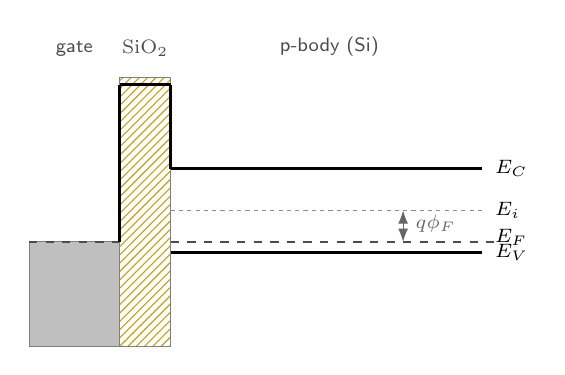
\begin{tikzpicture}[x=0.72cm,y=0.95cm]
% gate metallico
\fill[black!25] (0,-1.4) rectangle (1.6,0);
\draw[black!50,line width=0.3pt] (0,-1.4) rectangle (1.6,0);
\draw[Ef] (0,0) -- (1.6,0);
\node[reglab,anchor=south] at (0.8,2.35) {gate};
% ossido
\fill[pattern=north east lines, pattern color=oxcol] (1.6,-1.4) rectangle (2.5,2.2);
\draw[black!50,line width=0.3pt] (1.6,-1.4) rectangle (2.5,2.2);
\node[reglab,anchor=south] at (2.05,2.35) {$\mathrm{SiO_2}$};
\node[reglab,anchor=south] at (5.3,2.35) {p-body (Si)};
% bande silicio (flat band)
\draw[Eband] (2.5,0.98) -- (8.0,0.98);
\draw[Emid]  (2.5,0.42) -- (8.0,0.42);
\draw[Eband] (2.5,-0.14) -- (8.0,-0.14);
\draw[Ef] (2.5,0) -- (8.2,0);
% barriera ossido (scala ridotta)
\draw[Eband] (1.6,2.10) -- (2.5,2.10);
\draw[Eband] (1.6,2.10) -- (1.6,0);
\draw[Eband] (2.5,2.10) -- (2.5,0.98);
\node[enlab,anchor=west] at (8.05,0.98) {$E_C$};
\node[enlab,anchor=west] at (8.05,-0.14) {$E_V$};
\node[enlab,anchor=west] at (8.05,0.42) {$E_i$};
\node[enlab,anchor=west] at (8.05,0.06) {$E_F$};
\draw[<->,>=Latex,black!60,line width=0.4pt] (6.6,0.42) -- (6.6,0);
\node[enlab,anchor=west,black!60] at (6.65,0.24) {$q\phi_F$};
\end{tikzpicture}
\caption{$V_{GE}=0$: bande piatte, superficie di tipo p, nessun canale.}
\end{subfigure}\hfill
\begin{subfigure}[t]{0.48\textwidth}
\centering
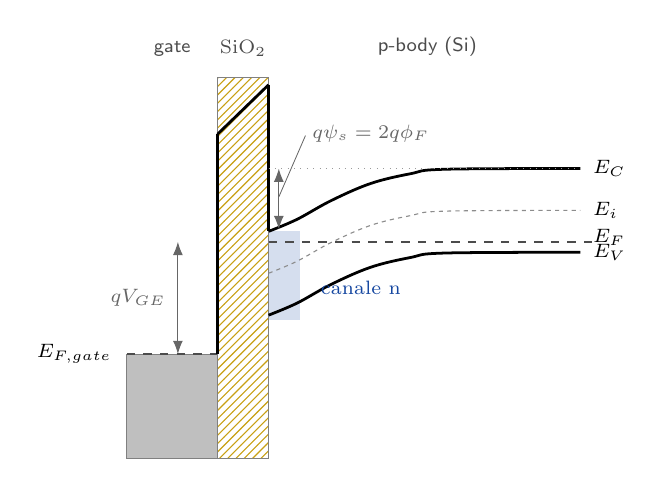
\begin{tikzpicture}[x=0.72cm,y=0.95cm]
% gate metallico portato a -qVge
\fill[black!25] (0,-2.9) rectangle (1.6,-1.5);
\draw[black!50,line width=0.3pt] (0,-2.9) rectangle (1.6,-1.5);
\draw[Ef] (0,-1.5) -- (1.6,-1.5);
\node[enlab,anchor=east] at (-0.1,-1.5) {$E_{F,gate}$};
\node[reglab,anchor=south] at (0.8,2.35) {gate};
% ossido
\fill[pattern=north east lines, pattern color=oxcol] (1.6,-2.9) rectangle (2.5,2.2);
\draw[black!50,line width=0.3pt] (1.6,-2.9) rectangle (2.5,2.2);
\node[reglab,anchor=south] at (2.05,2.35) {$\mathrm{SiO_2}$};
\node[reglab,anchor=south] at (5.3,2.35) {p-body (Si)};
% strato di inversione
\fill[ncol!18] (2.5,-1.05) rectangle (3.05,0.15);
% bande piegate
\draw[Eband] plot[smooth,tension=0.6] coordinates
  {(2.5,0.14) (3.0,0.30) (3.6,0.55) (4.3,0.78) (5.0,0.91) (5.6,0.97) (8.0,0.98)};
\draw[Emid,shift={(0,-0.56)}] plot[smooth,tension=0.6] coordinates
  {(2.5,0.14) (3.0,0.30) (3.6,0.55) (4.3,0.78) (5.0,0.91) (5.6,0.97) (8.0,0.98)};
\draw[Eband,shift={(0,-\EG)}] plot[smooth,tension=0.6] coordinates
  {(2.5,0.14) (3.0,0.30) (3.6,0.55) (4.3,0.78) (5.0,0.91) (5.6,0.97) (8.0,0.98)};
\draw[Ef] (2.5,0) -- (8.2,0);
% barriera ossido inclinata (scala ridotta)
\draw[Eband] (1.6,1.44) -- (2.5,2.10);
\draw[Eband] (1.6,1.44) -- (1.6,-1.5);
\draw[Eband] (2.5,2.10) -- (2.5,0.14);
\node[enlab,anchor=west] at (8.05,0.98) {$E_C$};
\node[enlab,anchor=west] at (8.05,-0.14) {$E_V$};
\node[enlab,anchor=west] at (8.05,0.42) {$E_i$};
\node[enlab,anchor=west] at (8.05,0.06) {$E_F$};
% quote
\draw[black!40,line width=0.3pt,dotted] (2.5,0.98) -- (8.0,0.98);
\draw[<->,>=Latex,black!60,line width=0.4pt] (2.68,0.98) -- (2.68,0.17);
\draw[black!60,line width=0.3pt] (2.68,0.60) -- (3.15,1.42);
\node[enlab,anchor=west,black!60] at (3.1,1.45) {$q\psi_s=2q\phi_F$};
\draw[<->,>=Latex,black!60,line width=0.4pt] (0.9,0) -- (0.9,-1.5);
\node[enlab,anchor=east,black!60] at (0.85,-0.75) {$qV_{GE}$};
\node[enlab,ncol,anchor=west] at (3.25,-0.62) {canale n};
\end{tikzpicture}
\caption{$V_{GE}>V_{th}$: inversione forte, $E_F$ sopra $E_i$ in superficie.}
\end{subfigure}
\caption{Diagramma a bande della struttura MOS (taglio trasversale
gate--ossido--p-body). Il livello di Fermi del semiconduttore resta unico e
orizzontale (corrente trasversale nulla); quello del gate e' abbassato di
$qV_{GE}$. L'altezza della barriera dell'ossido ($3{,}1$~eV rispetto a $E_C$
del silicio) e' rappresentata in scala ridotta.}
\label{fig:mos}
\end{figure}

\section{Stato di conduzione (\texorpdfstring{$V_{GE}>V_{th}$, $V_{CE}$ piccola}{VGE>Vth, VCE piccola})}

Con il canale formato la sequenza degli eventi e' la seguente:

\begin{enumerate}[nosep,leftmargin=1.6em]
  \item gli \textbf{elettroni} fluiscono dalla sorgente $\mathrm{n^{+}}$
        attraverso il canale di inversione e raggiungono la drift
        $\mathrm{n^{-}}$; questa corrente e' la corrente di base del PNP;
  \item la giunzione $J_1$ ($\mathrm{p^{+}}$/buffer) si porta in
        \textbf{polarizzazione diretta} ($\approx 0{,}7$~V) e inietta
        \textbf{lacune} nella drift;
  \item nella drift si stabilisce un plasma elettrone--lacuna quasi neutro con
        $n \simeq p \gg N_D$ (\emph{modulazione della conduttivita'});
  \item le lacune attraversano la drift, vengono raccolte dalla giunzione $J_2$
        (polarizzata inversamente) ed escono dal contatto di emettitore
        attraverso il p-body.
\end{enumerate}

Sul diagramma a bande (Fig.~\ref{fig:on}) questo si legge cosi':

\begin{itemize}[nosep,leftmargin=1.4em]
  \item la barriera $\mathrm{n^{+}}$/p-body \textbf{scompare} lungo il cammino
        superficiale, perche' la superficie del body e' invertita: e' il canale;
  \item nella drift i due quasi-livelli sono \textbf{separati di circa
        $0{,}7$--$0{,}8$~eV}, con $E_{Fn}>E_{Fp}$: e' la firma dell'alta
        iniezione,
        \begin{equation}
        n\,p = n_i^2 \exp\!\left(\frac{E_{Fn}-E_{Fp}}{kT}\right)
        \;\Rightarrow\;
        n \simeq p \sim 10^{16}\!-\!10^{17}~\mathrm{cm^{-3}} \gg N_D;
        \end{equation}
  \item entrambi i quasi-livelli sono \textbf{leggermente inclinati} attraverso
        la drift: e' la caduta ohmica residua, tanto piu' piccola quanto piu'
        denso e' il plasma (e infatti $E_{Fn}$ ed $E_{Fp}$ restano quasi
        paralleli);
  \item sulla giunzione $J_1$ i quasi-livelli si separano di $qV_{J1}$: e' la
        soglia di ginocchio che rende $V_{CE(sat)}$ non nulla a corrente nulla.
\end{itemize}

Il bilancio complessivo e'

\begin{equation}
V_{CE(sat)} \;=\; V_{J1}\;+\;V_{drift}\;+\;V_{canale}
\;\approx\; 0{,}7\!-\!0{,}9~\mathrm{V} \;+\; \text{(qualche 0,1~V)} \;+\; I_C R_{ch},
\end{equation}

dove la separazione $E_{Fn}-E_{Fp}$ ai due terminali metallici vale
esattamente $qV_{CE}$: i quasi-livelli devono infatti ricongiungersi al livello
di Fermi unico del metallo su ciascun contatto ohmico.

\begin{figure}[H]
\centering
\def\EcOn{(0,0.06) (0.8,0.06) (1.0,0.16) (1.3,0.12) (1.8,0.08) (2.2,0.04)
           (2.6,0.01) (3.0,0.04) (3.6,0.00) (5.0,-0.19) (6.5,-0.38)
           (7.6,-0.52) (8.2,-0.58) (8.6,-0.66) (9.0,-0.70) (9.2,-0.68)
           (9.5,-0.52) (9.8,-0.50) (10.8,-0.50)}
\begin{tikzpicture}[x=0.88cm,y=1.55cm]
\foreach \x in {1.0,2.6,8.2,9.0} \draw[sep] (\x,-1.88) -- (\x,0.45);
\node[reglab] at (0.5,0.60)  {$\mathrm{n^{+}}$};
\node[reglab] at (1.8,0.60)  {canale};
\node[reglab] at (5.4,0.60)  {$\mathrm{n^{-}}$ drift (plasma $n\simeq p$)};
\node[reglab] at (8.6,0.60)  {buffer};
\node[reglab] at (9.9,0.60)  {$\mathrm{p^{+}}$};
% bande
\draw[Eband] plot[smooth,tension=0.55] coordinates {\EcOn};
\draw[Eband,shift={(0,-\EG)}] plot[smooth,tension=0.55] coordinates {\EcOn};
\draw[Emid,shift={(0,-0.56)}] plot[smooth,tension=0.55] coordinates {\EcOn};
% quasi livelli
\draw[Efn] plot[smooth,tension=0.6] coordinates
  {(-0.2,0) (0.9,0) (1.3,-0.02) (2.0,-0.06) (2.6,-0.10) (3.2,-0.14)
   (5.0,-0.35) (7.0,-0.60) (8.2,-0.72) (9.0,-0.78) (9.4,-0.88) (10.0,-1.25)
   (10.8,-1.50)};
\draw[Efp] plot[smooth,tension=0.6] coordinates
  {(-0.2,0) (1.0,0) (2.2,-0.03) (2.6,-0.06) (2.9,-0.40) (3.3,-0.85)
   (3.8,-0.92) (5.0,-1.08) (6.5,-1.25) (8.2,-1.44) (9.0,-1.48) (10.0,-1.50)
   (10.8,-1.50)};
% etichette
\node[enlab,anchor=east,ncol] at (-0.25,0.14) {$E_{Fn}$};
\node[enlab,anchor=east,pcol] at (-0.25,-0.16) {$E_{Fp}$};
\node[enlab,anchor=west] at (10.9,-0.50) {$E_C$};
\node[enlab,anchor=west] at (10.9,-1.62) {$E_V$};
\node[enlab,anchor=west,ncol,fill=white,inner sep=1pt] at (7.05,-0.53) {$E_{Fn}$};
\node[enlab,anchor=west,pcol,fill=white,inner sep=1pt] at (6.55,-1.35) {$E_{Fp}$};
% quota separazione nel plasma
\draw[<->,>=Latex,black!60,line width=0.4pt] (4.4,-0.30) -- (4.4,-1.02);
\node[enlab,anchor=east,black!60,align=right,fill=white,inner sep=1.5pt] at (4.3,-0.66)
  {$E_{Fn}\!-\!E_{Fp}$\\[-1pt]$\approx 0{,}75$~eV};
% quota qVce
\draw[<->,>=Latex,black!60,line width=0.4pt] (10.55,0) -- (10.55,-1.50);
\draw[black!40,line width=0.3pt,dotted] (-0.2,0) -- (10.55,0);
\node[enlab,anchor=east,black!60] at (10.5,-0.14) {$qV_{CE}$};
% flussi
\draw[eflow] (1.4,0.30) -- (3.4,0.30);
\node[enlab,ncol,anchor=south] at (2.4,0.31) {elettroni};
\draw[hflow] (8.6,-2.02) -- (6.4,-2.02);
\node[enlab,pcol,anchor=north] at (7.5,-2.01) {lacune};
\end{tikzpicture}
\caption{Stato di conduzione, lungo il cammino di corrente
$\mathrm{n^{+}}\!\to$ canale di inversione $\to$ drift $\to$ buffer $\to
\mathrm{p^{+}}$. I quasi-livelli sono separati di $\approx 0{,}75$~eV in tutta
la drift (alta iniezione) e la loro pendenza, ridotta dalla modulazione della
conduttivita', rappresenta la caduta ohmica. Ai contatti la separazione totale
vale $qV_{CE}$. In prossimita' di $J_2$ l'andamento di $E_{Fp}$ e' schematico:
le lacune vengono raccolte dal p-body ed $E_{Fp}$ si ricongiunge al livello di
Fermi dell'emettitore.}
\label{fig:on}
\end{figure}

\section{Spegnimento e coda di corrente}

Quando $V_{GE}$ scende sotto $V_{th}$ il canale scompare e la corrente di
elettroni si interrompe quasi istantaneamente. Il plasma immagazzinato nella
drift, pero', non ha alcun percorso di estrazione: la sua separazione
$E_{Fn}-E_{Fp}$ si annulla solo per \emph{ricombinazione}, con costante di
tempo pari alla vita media dei portatori $\tau$. Questo si traduce nella
caratteristica coda di corrente ($I_{tail}$), che domina le perdite di
spegnimento. Le tecniche di controllo della vita media (irraggiamento
elettronico, drogaggio con oro/platino) e le strutture field-stop agiscono
proprio sulla quantita' di plasma e sulla sua velocita' di estinzione,
imponendo il classico compromesso $V_{CE(sat)}$ contro $E_{off}$.

\section{Quadro riassuntivo}

\begin{table}[H]
\centering
\footnotesize
\begin{tabular}{@{}p{0.18\textwidth}p{0.235\textwidth}p{0.235\textwidth}p{0.25\textwidth}@{}}
\toprule
 & \textbf{Riposo} & \textbf{Blocco} & \textbf{Conduzione}\\
 & $V_{GE}=0$, $V_{CE}=0$ & $V_{GE}=0$, $V_{CE}>0$ & $V_{GE}>V_{th}$, $V_{CE}$ piccola\\
\midrule
Livelli di Fermi & $E_F$ unico, orizzontale & $E_{Fn}$, $E_{Fp}$ separati di $qV_{CE}$ & $E_{Fn}$, $E_{Fp}$ separati di $qV_{CE}$\\
Superficie del body & tipo p & tipo p (o svuotata) & invertita (canale n)\\
Giunzione $J_2$ (body/drift) & equilibrio & inversa, sostiene $V_{CE}$ & lievemente inversa, raccoglie lacune\\
Giunzione $J_1$ ($\mathrm{p^{+}}$/buffer) & equilibrio & quasi non polarizzata & diretta, inietta lacune\\
Drift $\mathrm{n^{-}}$ & $np=n_i^2$ & $np \ll n_i^2$ (svuotata) & $np \gg n_i^2$ (alta iniezione)\\
Corrente & nulla & $I_{CES}$ di generazione & $I_C$, elettroni + lacune\\
\bottomrule
\end{tabular}
\caption{Sintesi dei tre stati operativi letti attraverso i livelli di Fermi.}
\end{table}

\section*{Nota sui valori usati nei disegni}
\small
I diagrammi sono qualitativi ma internamente coerenti. Valori adottati:
$E_g = 1{,}12$~eV, $N_A(\text{body}) \approx 10^{17}~\mathrm{cm^{-3}}$
($\phi_F \approx 0{,}42$~V), $N_D(\text{drift})$ molto basso
($E_C-E_F \approx 0{,}25$~eV), buffer e $\mathrm{n^{+}}$ degeneri o quasi.
Nelle Fig.~\ref{fig:block} e \ref{fig:on} la tensione $V_{CE}$ e' disegnata
rispettivamente pari a $2$~V e $1{,}5$~V: la prima e' fortemente ridotta
rispetto ai valori reali di blocco (centinaia di volt) per poter rappresentare
le bande sulla stessa scala verticale del gap.

\end{document}
